\documentclass[11pt, oneside]{article}   	% use "amsart" instead of "article" for AMSLaTeX format
\usepackage{geometry}                		% See geometry.pdf to learn the layout options. There are lots.
\usepackage{mathtools}
\usepackage{graphicx}
\geometry{letterpaper}                   		% ... or a4paper or a5paper or ... 
%\geometry{landscape}                		% Activate for rotated page geometry
%\usepackage[parfill]{parskip}    		% Activate to begin paragraphs with an empty line rather than an indent
\usepackage{graphicx}				% Use pdf, png, jpg, or eps§ with pdflatex; use eps in DVI mode
								% TeX will automatically convert eps --> pdf in pdflatex		
\usepackage{amssymb}

%SetFonts

%SetFonts


\title{Bi-Directional Training in Interference Network}
\author{Shao-Han Chen}
%\date{}							% Activate to display a given date or no date

\begin{document}
\maketitle
%\section{}
%\subsection{}

1. Optimization Problem
\begin{align*}
\min_{v_{i} , g_{i}} \displaystyle\sum_{i} MSE^{(c)}_{i}+MSE^{(p)}_{i}
\end{align*}

2. The received signal vector at k-th receiver
\begin{align*}
\textbf{y}_{k} &= \textbf{H}_{kk}
			(\textbf{v}^{(c)}_{k}x
			+\textbf{v}^{(p)}_{k}x^{(p)}_{k})
			+\displaystyle\sum_{j \neq k}\textbf{H}_{kj}(\textbf{v}^{(c)}_{j}x+\textbf{v}^{(p)}_{j}x^{(p)}_{j})
			+\textbf{n}_{k}
\end{align*}

3. SINR Derivation
\begin{align*}
s^{(c)}_{k} = \textbf{g}^{H(c)}_{k}
		(\displaystyle\sum_{i}
		\textbf{H}_{ki} 
		\textbf{v}^{(c)}_{i}x)
\end{align*}

\begin{align*}
s^{(p)}_{k} = \textbf{g}^{H(p)}_{k}
		(\textbf{H}_{kk} 
		\textbf{v}^{(p)}_{k}x^{(p)}_{k})
\end{align*}

\begin{align*}
n^{(c)}_{k} = \textbf{g}^{H(c)}_{k}
		(\displaystyle\sum_{i}
		\textbf{H}_{ki} 
		\textbf{v}^{(p)}_{i}x^{(p)}_{i}
		+\textbf{n}_{k})
\end{align*}

\begin{align*}
n^{(p)}_{k} = \textbf{g}^{H(p)}_{k}
		(\displaystyle\sum_{i}
		\textbf{H}_{ki} 
		\textbf{v}^{(c)}_{i}x
		+\displaystyle\sum_{j \neq k}\textbf{H}_{kj}\textbf{v}^{(p)}_{j}x^{(p)}_{j}
		+\textbf{n}_{k})
\end{align*}

\begin{align*}
\frac	{	|s^{(c)}_{k}|^2	}{	|n^{(c)}_{k}|^2	} = 
\frac {	|\textbf{g}^{H(c)}_{k}
		\displaystyle\sum_{i}
		\textbf{H}_{ki} 
		\textbf{v}^{(c)}_{i}|^2	
	} 
	{	\displaystyle\sum_{i}
		|\textbf{g}^{H(c)}_{k}
		\textbf{H}_{ki} 
		\textbf{v}^{(p)}_{i}|^2
		+|\textbf{g}^{H(c)}_{k}
		\textbf{R}_{k}
		\textbf{g}^{(c)}_{k}|
	}
\end{align*}

\begin{align*}
\frac	{	|s^{(p)}_{k}|^2	}{	|n^{(p)}_{k}|^2	} = 
\frac {|\textbf{g}^{H(p)}_{k}
		\textbf{H}_{kk} 
		\textbf{v}^{(p)}_{k}|^2	
	} 
	{	|\textbf{g}^{H(p)}_{k}
		\displaystyle\sum_{i}
		\textbf{H}_{ki} 
		\textbf{v}^{(c)}_{i}|^2
		+\displaystyle\sum_{j \neq k}
		|\textbf{g}^{H(p)}_{k}
		\textbf{H}_{kj} 
		\textbf{v}^{(p)}_{j}|^2
		+|\textbf{g}^{H(p)}_{k}
		\textbf{R}_{k}
		\textbf{g}^{(p)}_{k}|
	}
\end{align*}

4. Max-SINR Algorithm[Gomadam,2011]
\begin{align*}
Forward\ Training (fix\  \textbf{v}^{(c)}_{k}, \textbf{v}^{(p)}_{k}, \forall k)
\end{align*}

\begin{align*}
\textbf{g}^{(c)}_{k} = 
&\bigg[
\textbf{H}_{kk}	\textbf{v}^{(c)}_{k}	\textbf{v}^{H(c)}_{k}	\textbf{H}^{H}_{kk}
+\textbf{H}_{kk}	\textbf{v}^{(p)}_{k}	\textbf{v}^{H(p)}_{k}	\textbf{H}^{H}_{kk}	\\
&+(\displaystyle\sum_{j \neq k}\textbf{H}_{kj}\textbf{v}^{(c)}_{j})
(\displaystyle\sum_{j \neq k}\textbf{v}^{H(c)}_{j}\textbf{H}^{H}_{kj})
+(\displaystyle\sum_{j \neq k}\textbf{H}_{kj}\textbf{v}^{(p)}_{j} \textbf{v}^{H(p)}_{j}\textbf{H}^{H}_{kj})	\\
&+\textbf{H}_{kk}	\textbf{v}^{(c)}_{k}
(\displaystyle\sum_{j \neq k}\textbf{v}^{H(c)}_{j}\textbf{H}^{H}_{kj})
+(\displaystyle\sum_{j \neq k}\textbf{H}_{kj}\textbf{v}^{(c)}_{j})
\textbf{v}^{H(c)}_{k}	\textbf{H}^{H}_{kk}
+\sigma^2	\textbf{I}
\bigg]^{-1}	 	(\displaystyle\sum_{i}	\textbf{H}_{ki} 	\textbf{v}^{(c)}_{i})	
\end{align*}

\begin{align*}
\textbf{g}^{(p)}_{k} = 	
&\bigg[
\textbf{H}_{kk}	\textbf{v}^{(c)}_{k}	\textbf{v}^{H(c)}_{k}	\textbf{H}^{H}_{kk}
+\textbf{H}_{kk}	\textbf{v}^{(p)}_{k}	\textbf{v}^{H(p)}_{k}	\textbf{H}^{H}_{kk}	\\
&+(\displaystyle\sum_{j \neq k}\textbf{H}_{kj}\textbf{v}^{(c)}_{j})
(\displaystyle\sum_{j \neq k}\textbf{v}^{H(c)}_{j}\textbf{H}^{H}_{kj})
+(\displaystyle\sum_{j \neq k}\textbf{H}_{kj}\textbf{v}^{(p)}_{j} \textbf{v}^{H(p)}_{j}\textbf{H}^{H}_{kj})	\\
&+\textbf{H}_{kk}	\textbf{v}^{(c)}_{k}
(\displaystyle\sum_{j \neq k}\textbf{v}^{H(c)}_{j}\textbf{H}^{H}_{kj})
+(\displaystyle\sum_{j \neq k}\textbf{H}_{kj}\textbf{v}^{(c)}_{j})
\textbf{v}^{H(c)}_{k}	\textbf{H}^{H}_{kk}
+\sigma^2	\textbf{I}
\bigg]^{-1}	 (\textbf{H}_{kk} 	\textbf{v}^{(p)}_{k})
\end{align*}

\begin{align*}
Backward\ Training (fix\  \textbf{g}^{(c)}_{k}, \textbf{g}^{(p)}_{k}, \forall k)
\end{align*}

\begin{align*}
\textbf{Z}_{ab}=\textbf{H}^{T}_{ba}
\end{align*}


\begin{align*}
without \ cooperation
\end{align*}

\begin{align*}
\textbf{v}^{(c)}_{k} = 
&\bigg[
\textbf{Z}_{kk}	\textbf{g}^{(c)}_{k}	\textbf{g}^{H(c)}_{k}	\textbf{Z}^{H}_{kk}
+\textbf{Z}_{kk}	\textbf{g}^{(p)}_{k}	\textbf{g}^{H(p)}_{k}	\textbf{Z}^{H}_{kk}	\\
&+(\displaystyle\sum_{j \neq k}\textbf{Z}_{kj}\textbf{g}^{(c)}_{j})
(\displaystyle\sum_{j \neq k}\textbf{g}^{H(c)}_{j}\textbf{Z}^{H}_{kj})
+(\displaystyle\sum_{j \neq k}\textbf{Z}_{kj}\textbf{g}^{(p)}_{j}	\textbf{g}^{H(p)}_{j}\textbf{Z}^{H}_{kj})	\\
&+\textbf{Z}_{kk}	\textbf{g}^{(c)}_{k}
(\displaystyle\sum_{j \neq k}\textbf{g}^{H(c)}_{j}\textbf{Z}^{H}_{kj})
+(\displaystyle\sum_{j \neq k}\textbf{Z}_{kj}\textbf{g}^{(c)}_{j})
\textbf{g}^{H(c)}_{k}	\textbf{Z}^{H}_{kk}
+\sigma^2	\textbf{I}
\bigg]
^{-1}	 (	\displaystyle\sum_{i}   \textbf{Z}_{ki} 	\textbf{g}^{(c)}_{i}	)
\end{align*}





\begin{align*}
with \ cooperation
\end{align*}

\begin{align*}
\textbf{V}^{(c)} =  		
&\left\{ 
\textbf{[Z]}	\textbf{g}^{(c)}	\textbf{g}^{H(c)}		\textbf{[Z]}^{H}
+\textbf{[Z]}
\begin{bmatrix}
       \textbf{g}^{(p)}_{1}	\textbf{g}^{H(p)}_{1} &  &   \textbf{O}      \\[0.3em]
        & \ddots       & \\[0.3em]
           \textbf{O}        & & \textbf{g}^{(p)}_{k}	\textbf{g}^{H(p)}_{k}
     \end{bmatrix}
    \textbf{[Z]}^{H}
    +\sigma^2	\textbf{I}
\right\}
^{-1} ( \textbf{[Z]}  \textbf{g}^{(c)}	)	
\end{align*}

\begin{align*}
\textbf{v}^{(p)}_{k} =	
 &\bigg[
\textbf{Z}_{kk}	\textbf{g}^{(c)}_{k}	\textbf{g}^{H(c)}_{k}	\textbf{Z}^{H}_{kk}
+\textbf{Z}_{kk}	\textbf{g}^{(p)}_{k}	\textbf{g}^{H(p)}_{k}	\textbf{Z}^{H}_{kk}	\\
&+(\displaystyle\sum_{j \neq k}\textbf{Z}_{kj}\textbf{g}^{(c)}_{j})
(\displaystyle\sum_{j \neq k}\textbf{g}^{H(c)}_{j}\textbf{Z}^{H}_{kj})
+(\displaystyle\sum_{j \neq k}\textbf{Z}_{kj}\textbf{g}^{(p)}_{j}	\textbf{g}^{H(p)}_{j}\textbf{Z}^{H}_{kj})	\\
&+\textbf{Z}_{kk}	\textbf{g}^{(c)}_{k}
(\displaystyle\sum_{j \neq k}\textbf{g}^{H(c)}_{j}\textbf{Z}^{H}_{kj})
+(\displaystyle\sum_{j \neq k}\textbf{Z}_{kj}\textbf{g}^{(c)}_{j})
\textbf{g}^{H(c)}_{k}	\textbf{Z}^{H}_{kk}
+\sigma^2	\textbf{I}
\bigg]^{-1}	 (\textbf{Z}_{kk}  \textbf{g}^{(p)}_{k})
\end{align*}

5. Bi-Directional Training with LMS Algorithm[Shi,2014]

\begin{align*}
Forward\ Training (fix\  \textbf{v}^{(c)}_{k}, \textbf{v}^{(p)}_{k}, \forall k)
\end{align*}

\begin{align*}
\textbf{g}^{(c)}_{k}(n+1)= \textbf{g}^{(c)}_{k}(n)+ \mu \textbf y_k(n) [x(n)- \textbf{g}^{H(c)}_{k}(n) \textbf y_k(n)]^*
\end{align*}

\begin{align*}
\textbf{g}^{(p)}_{k}(n+1)= \textbf{g}^{(p)}_{k}(n)+ \mu \textbf y_k(n) [x_k^{(p)}(n)- \textbf{g}^{H(p)}_{k}(n) \textbf y_k(n)]^*
\end{align*}

\begin{align*}
Backward\ Training (fix\  \textbf{g}^{(c)}_{k}, \textbf{g}^{(p)}_{k}, \forall k)(without\ cooperation)
\end{align*}

\begin{align*}
\textbf{v}^{(c)}_{k}(n+1)= \textbf{v}^{(c)}_{k}(n)+ \mu \textbf y_k(n) [x(n)- \textbf{v}^{H(c)}_{k}(n) \textbf y_k(n)]^*
\end{align*}

\begin{align*}
\textbf{v}^{(p)}_{k}(n+1)= \textbf{v}^{(p)}_{k}(n)+ \mu \textbf y_k(n) [x_k^{(p)}(n)- \textbf{v}^{H(p)}_{k}(n) \textbf y_k(n)]^*
\end{align*}

\begin{align*}
Backward\ Training (fix\  \textbf{g}^{(c)}_{k}, \textbf{g}^{(p)}_{k}, \forall k)(with\ cooperation)
\end{align*}

\begin{align*}
\textbf{V}^{(c)}(n+1)= \textbf{V}^{(c)}(n)+ \mu \textbf Y(n) [x(n)- \textbf{V}^{H(c)}(n) \textbf Y(n)	]^*
\end{align*}

\begin{align*}
\textbf{v}^{(p)}_{k}(n+1)= \textbf{v}^{(p)}_{k}(n)+ \mu \textbf y_k(n) [x_k^{(p)}(n)- \textbf{v}^{H(p)}_{k}(n) \textbf y_k(n)]^*
\end{align*}

6. Numerical Simulation(2 Users, 2X2 MIMO Channel)


\begin{align*}
Rayleigh\ Fading\ Channel
\end{align*}

\begin{align*}
\ Cross\ Channel\ Gain = 0.8*Direct\ Channel\ Gain
\end{align*}

\begin{align*}
SNR = \frac {1}{\sigma^2} = 10^3=30dB
\end{align*}

\begin{align*}
Observation1: &If\ the\ training\ length\ is\ long\ enough,\ each\ LMS\ filter\ (\textbf{v}^{(c)}_{k},\textbf{v}^{(p)}_{k},\textbf{g}^{(c)}_{k},\textbf{g}^{(p)}_{k},)\\
&will\ converge\ to\ Wiener\ filter
\end{align*}

\begin{align*}
Observation2:\ Use\ Wiener\ filters,\ and\ only\ send\ common\ messages.\ Sum\ rate\ C\ =\ 11.6\ bit/channel
\end{align*}

\begin{align*}
Observation3:\ Use\ Wiener\ filters,\ and\ only\ send\ private\ messages.\ Sum\ rate\ C\ =\ 2.63\ bit/channel
\end{align*}

\begin{align*}
Observation4:\ Use\ Wiener\ filters,\ and\  send\ both\ messages.\ Sum\ rate\ C\ =\ 3.35\ bit/channel
\end{align*}

\begin{align*}
Observation5:\ Under\ the\ cooperation\ scheme,\ transmitters\ don't\ converge\ to\ Wiener\ filters 
\end{align*}

\begin{align*}
Observation5:\ Under\ the\ cooperation\ scheme,\ C=3.15\ bit/channel
\end{align*}



\begin{figure}[bp!]
    \centering
    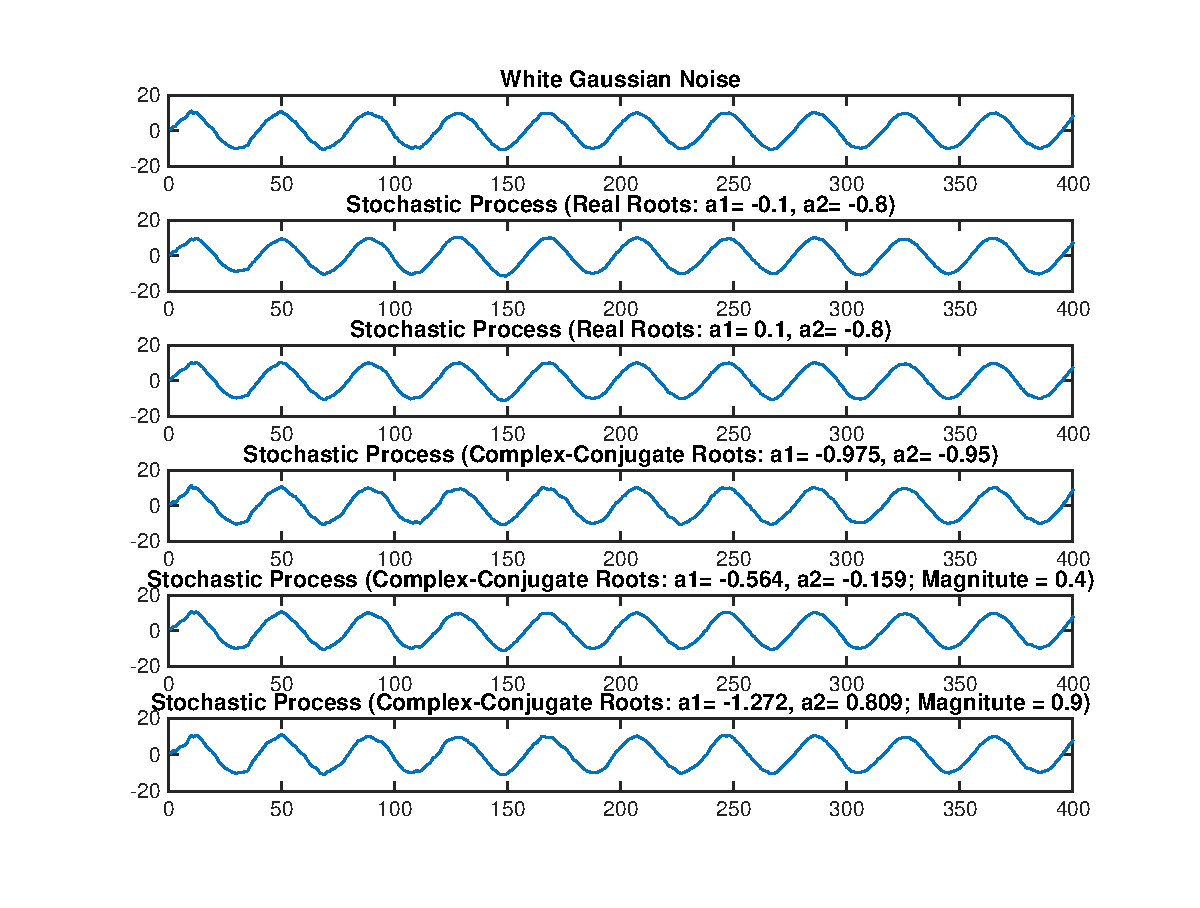
\includegraphics[width=150mm]{01}
    \caption{Insert caption}
\end{figure} 

\begin{figure}[bp!]
    \centering
    \centerline{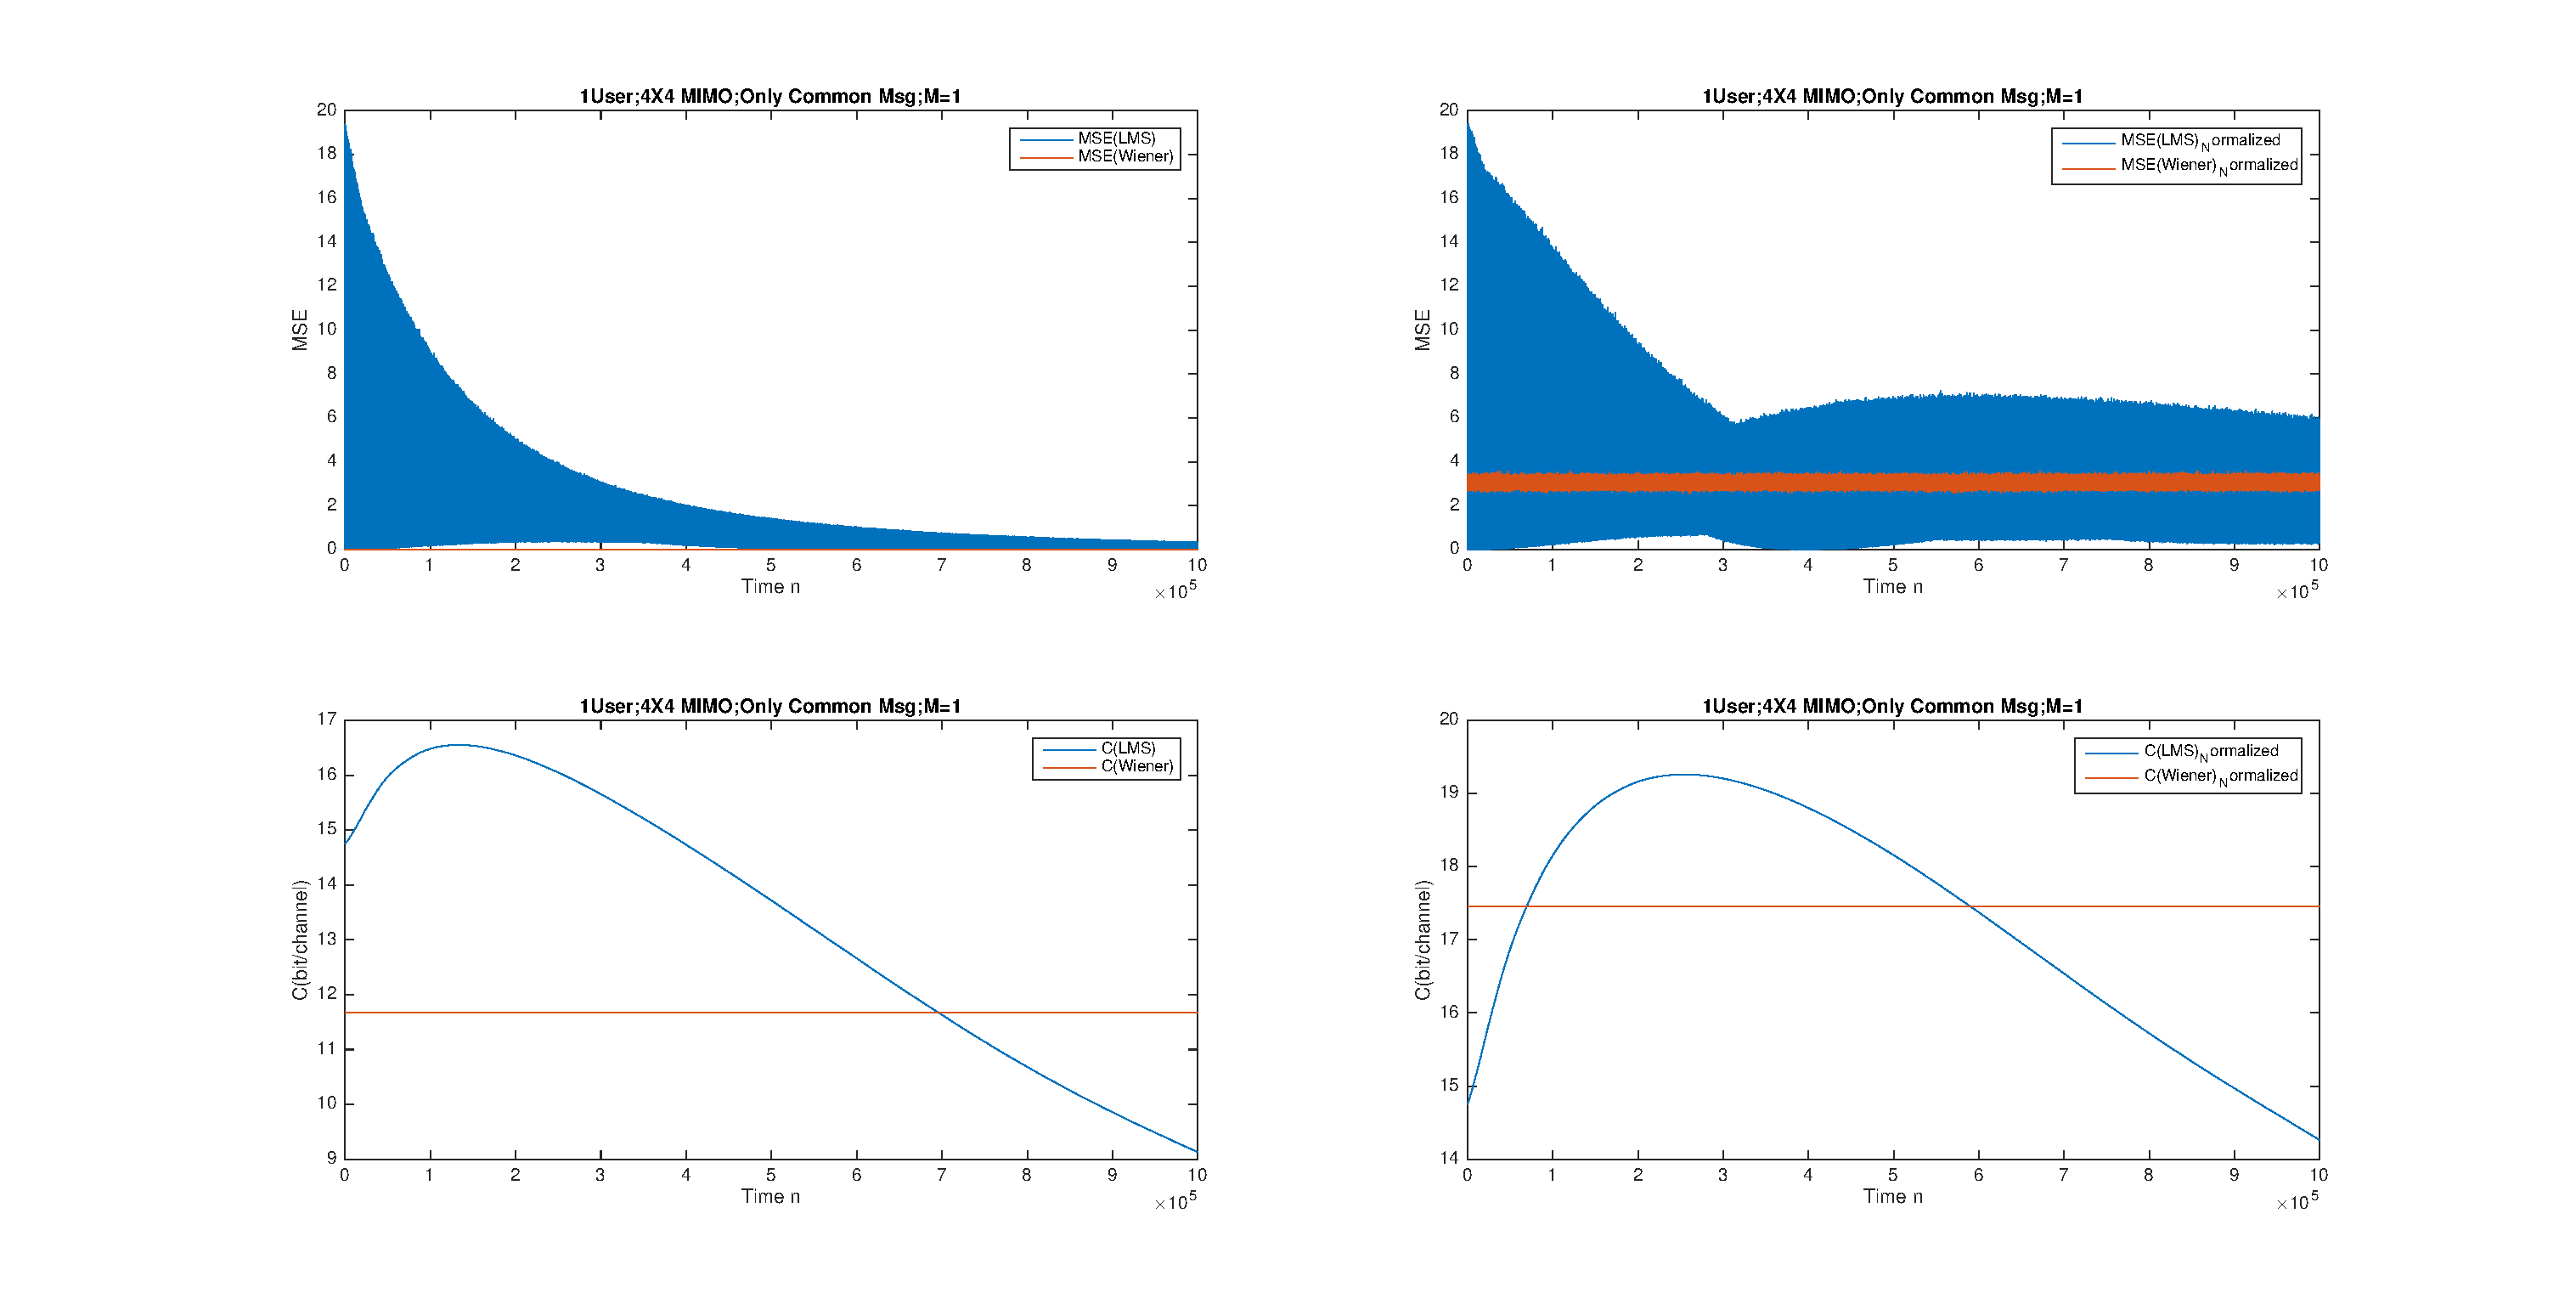
\includegraphics[width=220mm]{1USER_4X4MIMO}}
    \caption{Insert caption}
\end{figure} 

\begin{figure}[bp!]
    \centering
    \centerline{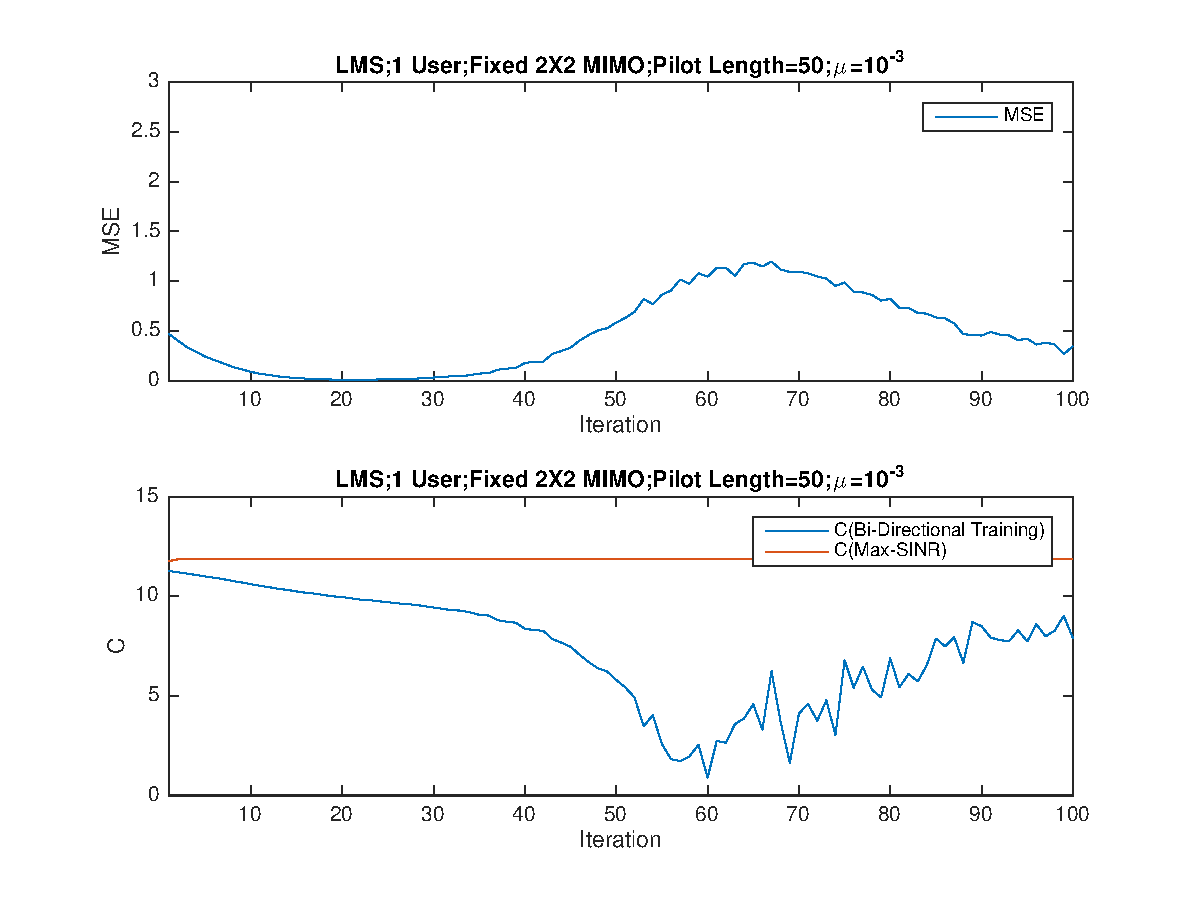
\includegraphics[width=220mm]{LMS1}}
    \caption{Insert caption}
\end{figure} 

\begin{figure}[bp!]
    \centering
    \centerline{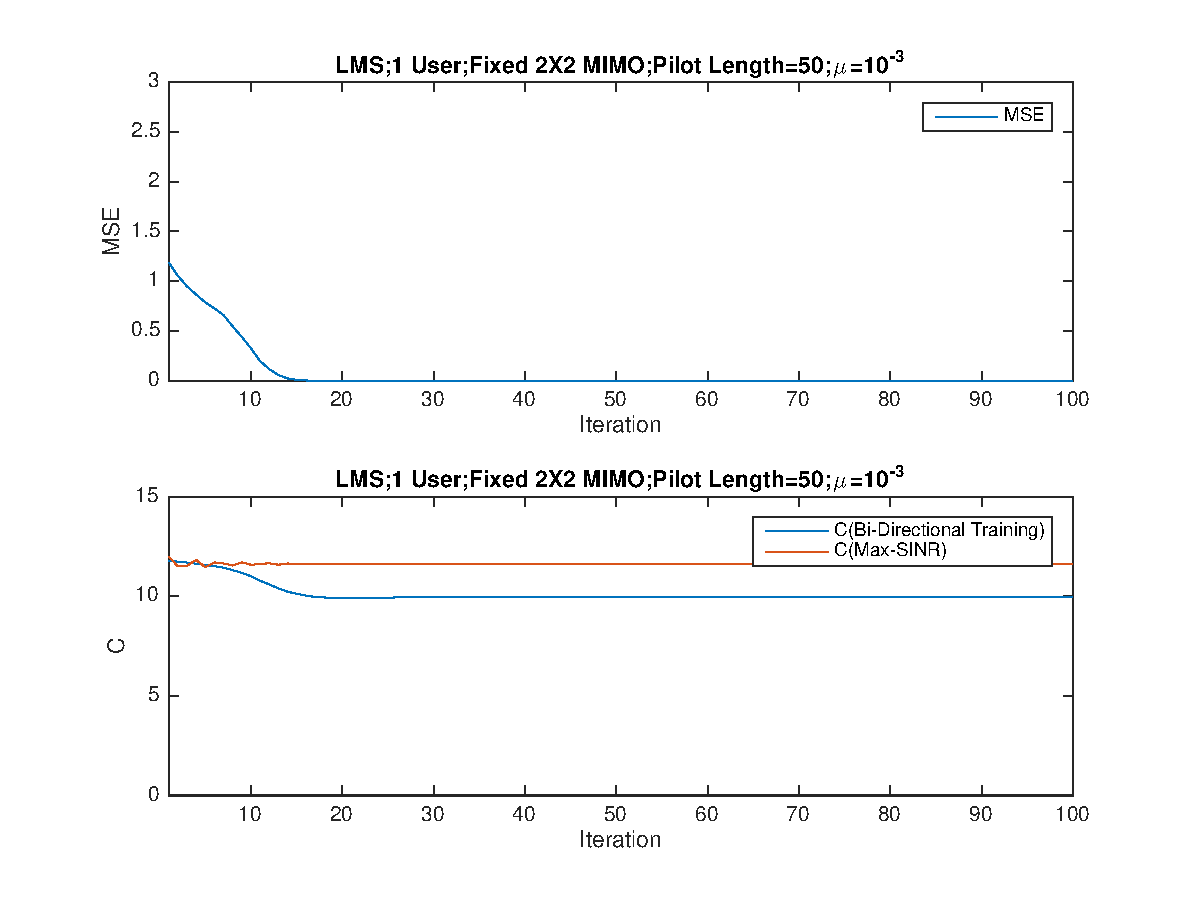
\includegraphics[width=220mm]{LMS2}}
    \caption{Insert caption}
\end{figure} 

\begin{figure}[bp!]
    \centering
    \centerline{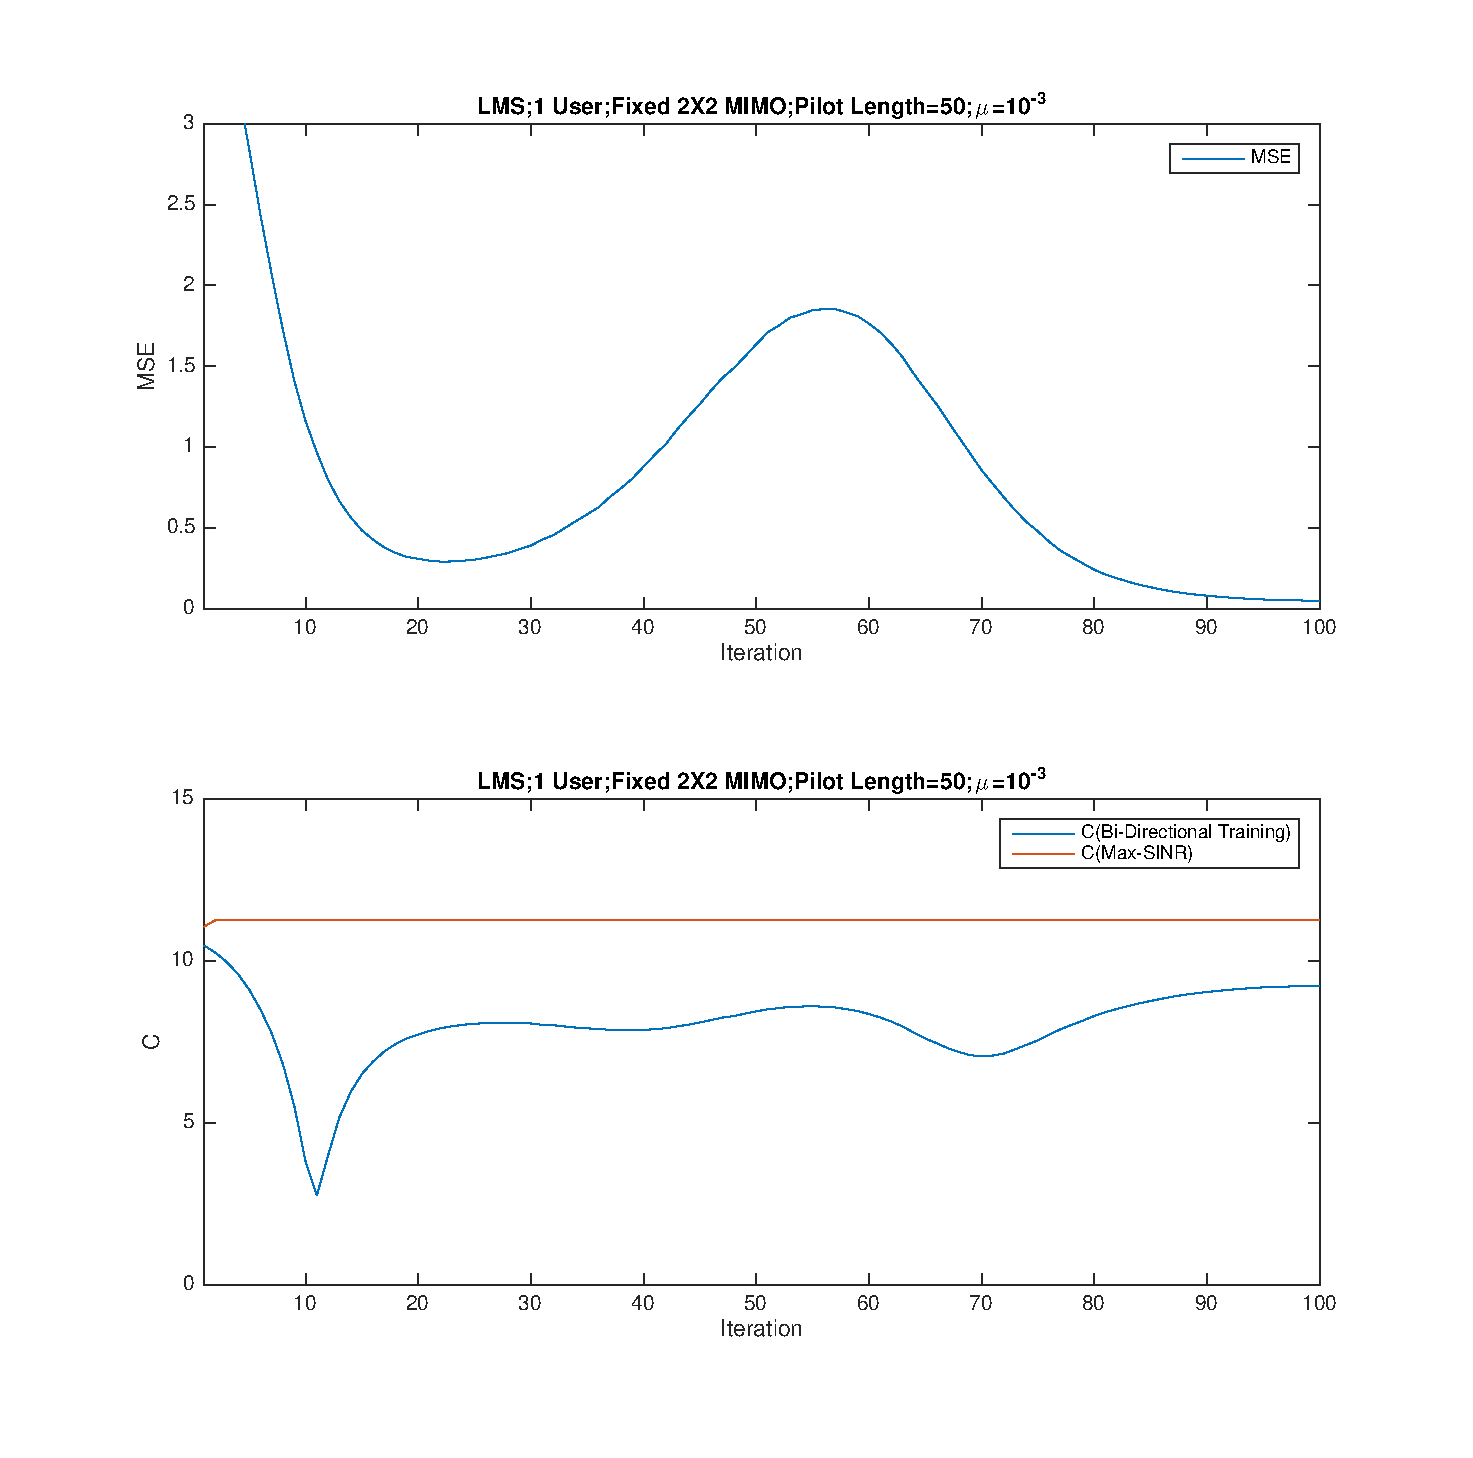
\includegraphics[width=220mm]{LMS3}}
    \caption{Insert caption}
\end{figure} 

\begin{figure}[bp!]
    \centering
    \centerline{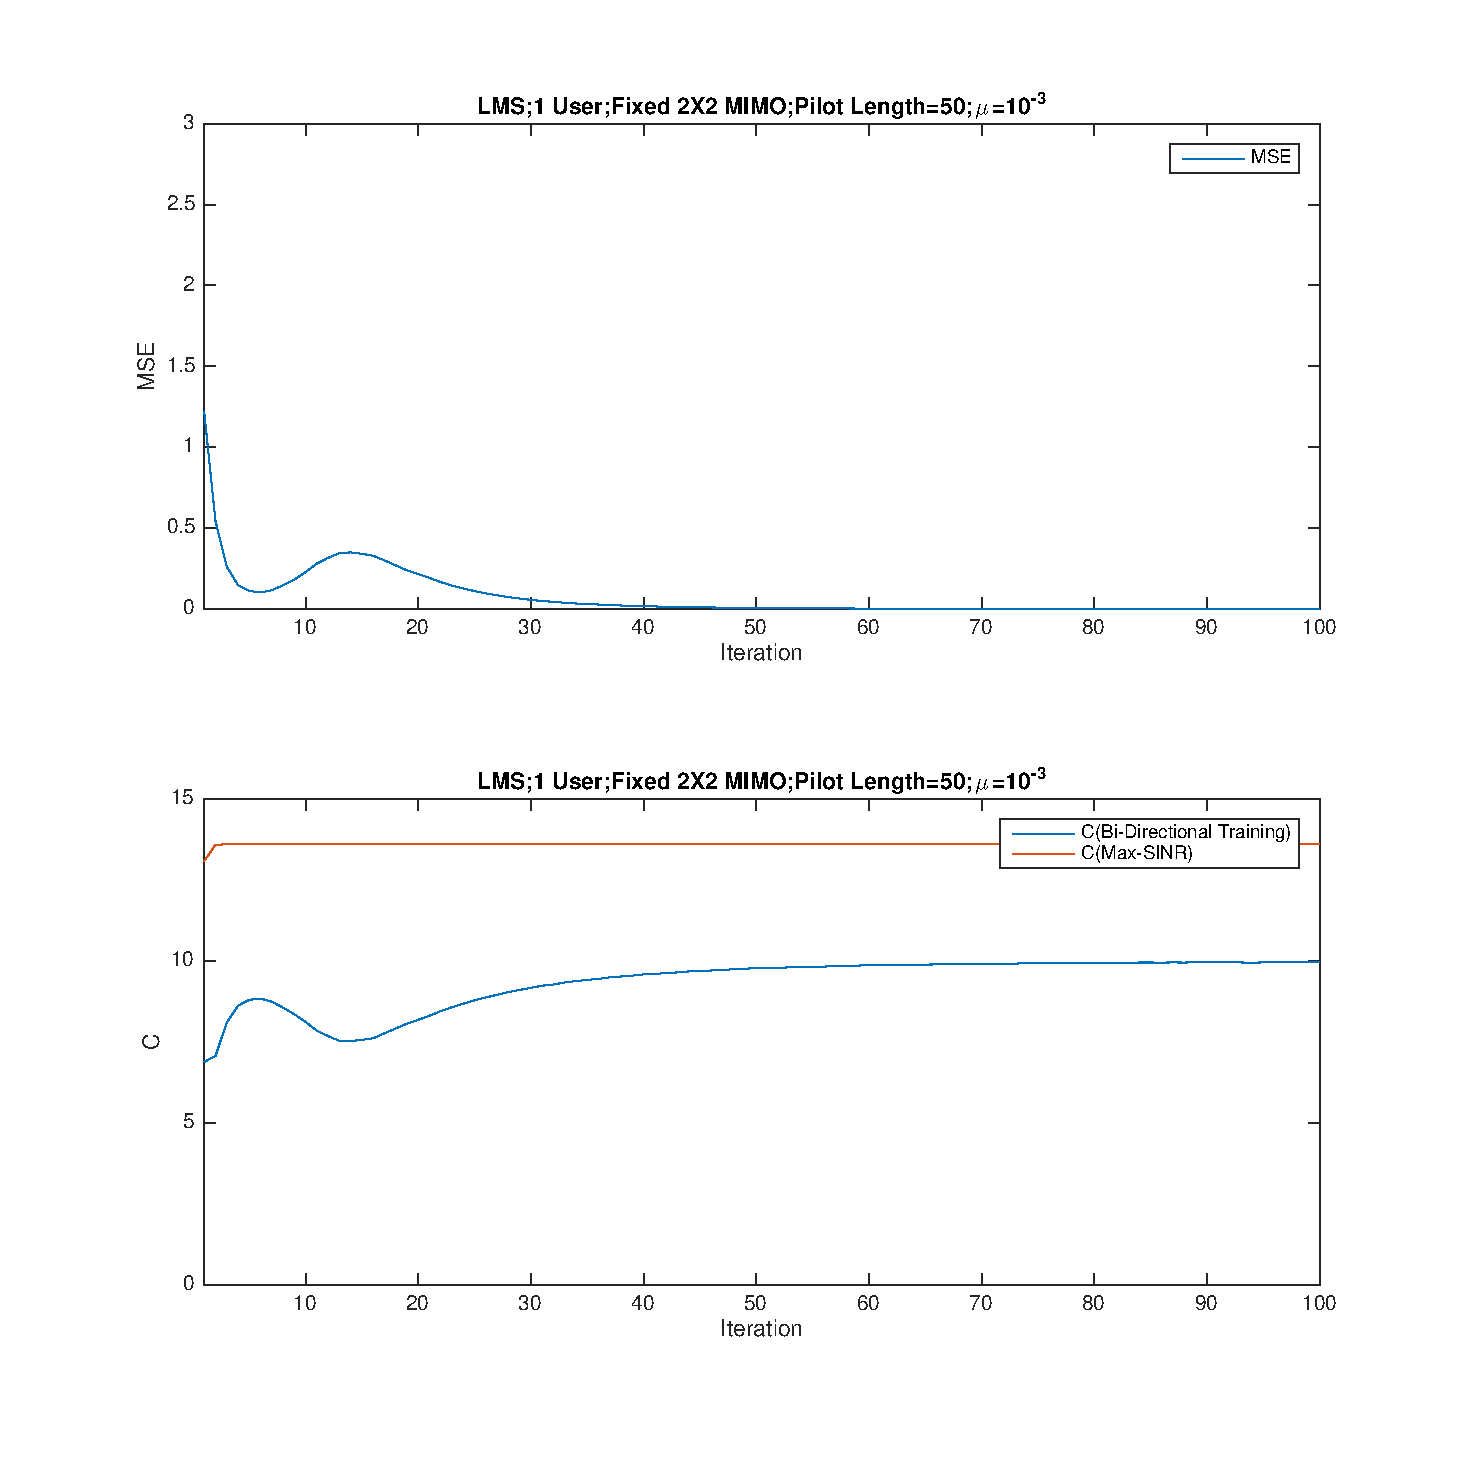
\includegraphics[width=220mm]{LMS4}}
    \caption{Insert caption}
\end{figure} 

\begin{figure}[bp!]
    \centering
    \centerline{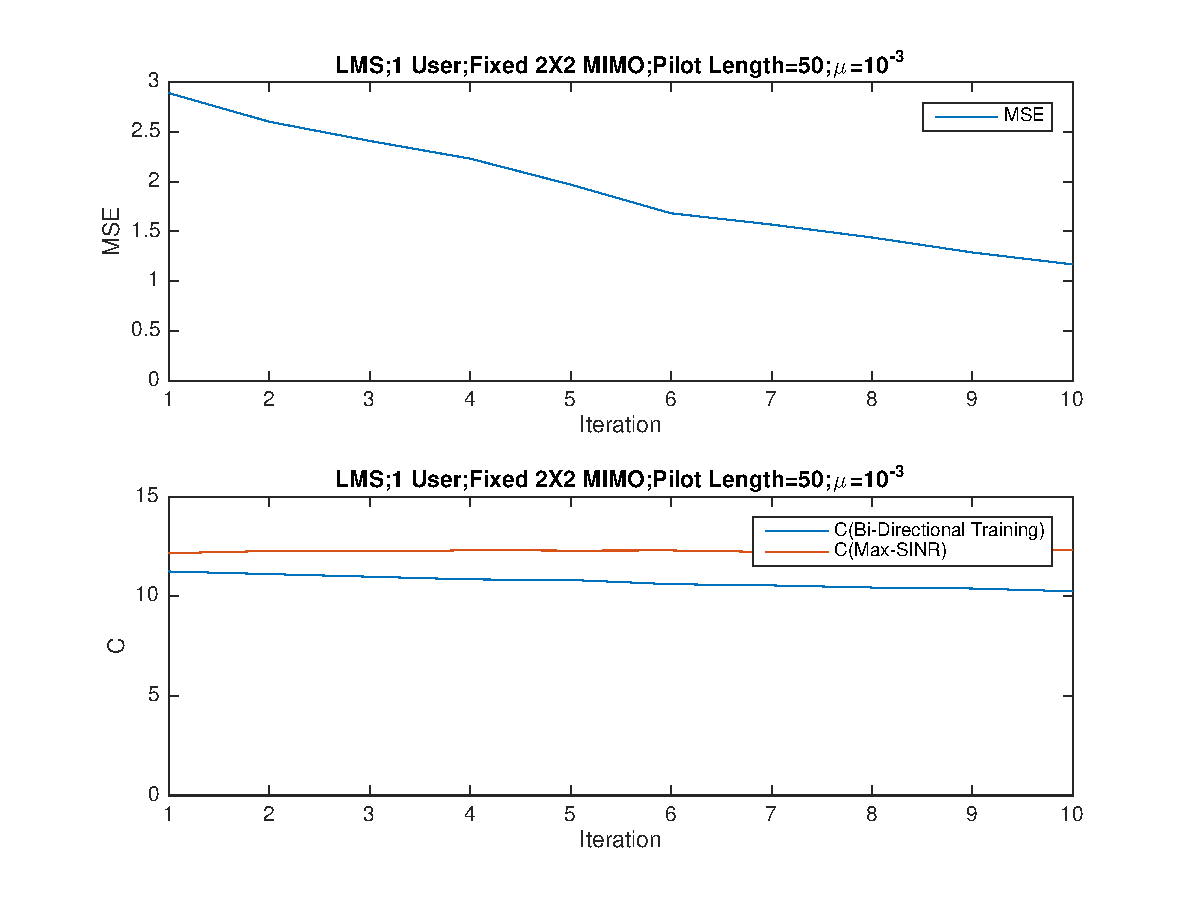
\includegraphics[width=220mm]{LMS5}}
    \caption{Insert caption}
\end{figure} 

\begin{figure}[bp!]
    \centering
    \centerline{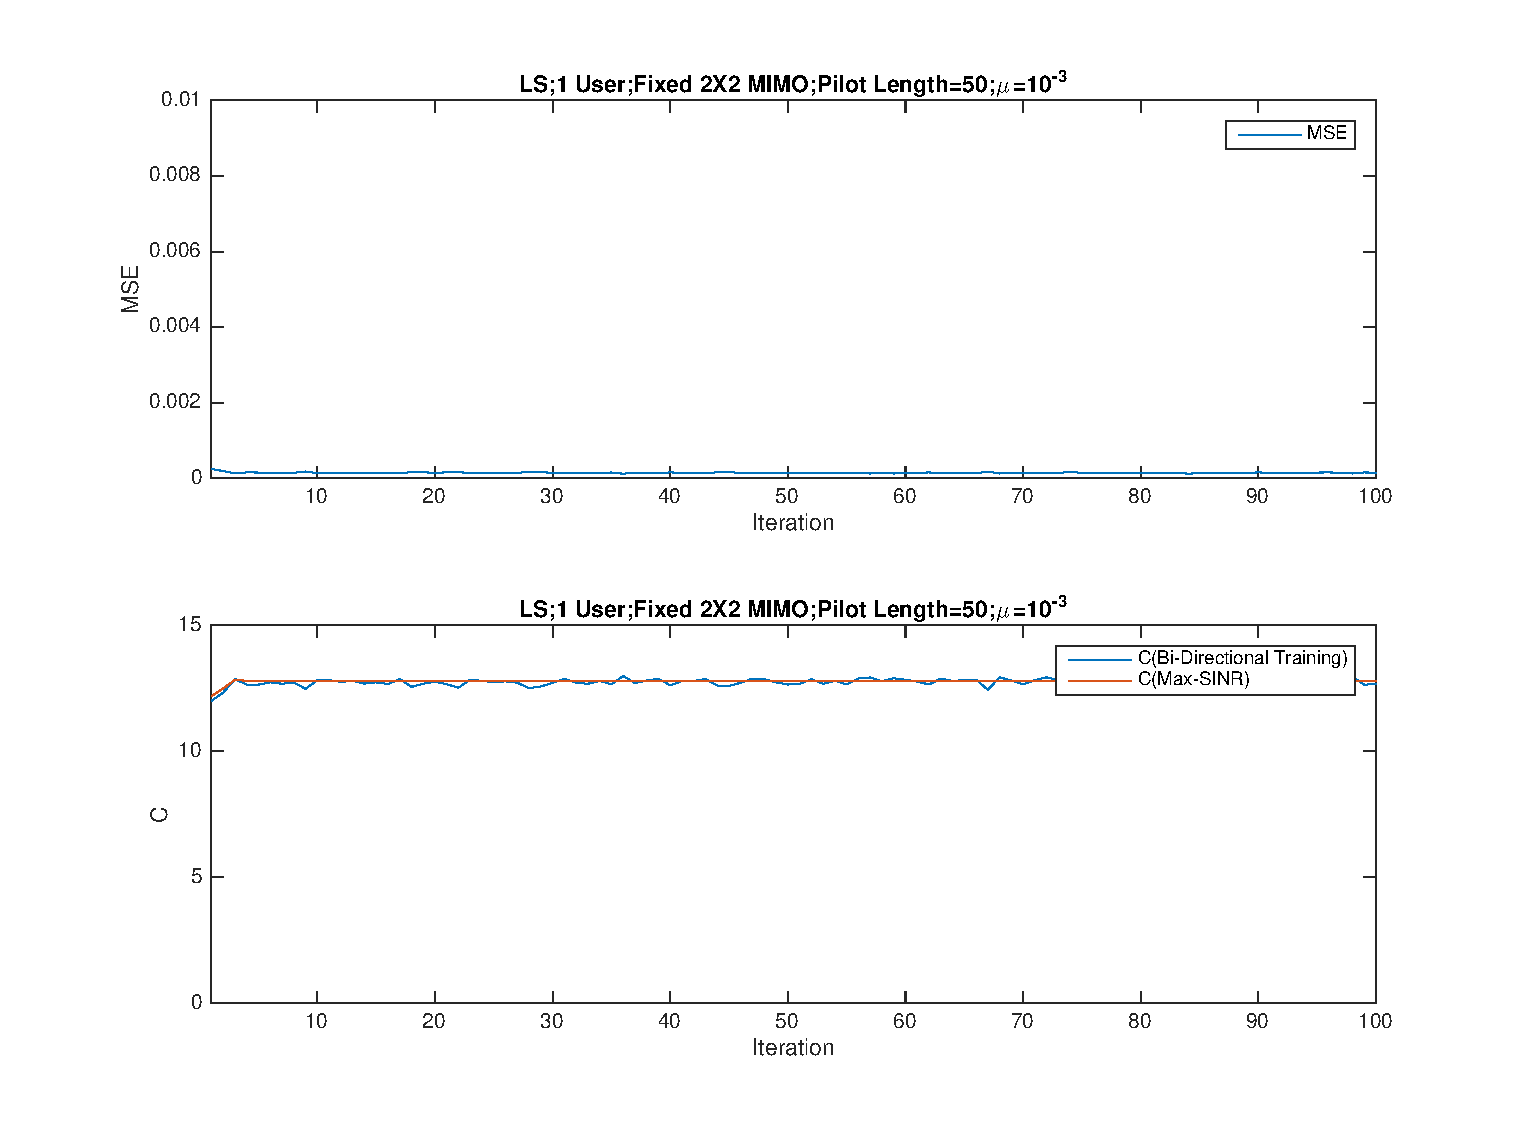
\includegraphics[width=220mm]{LS1}}
    \caption{Insert caption}
\end{figure} 

\begin{figure}[bp!]
    \centering
    \centerline{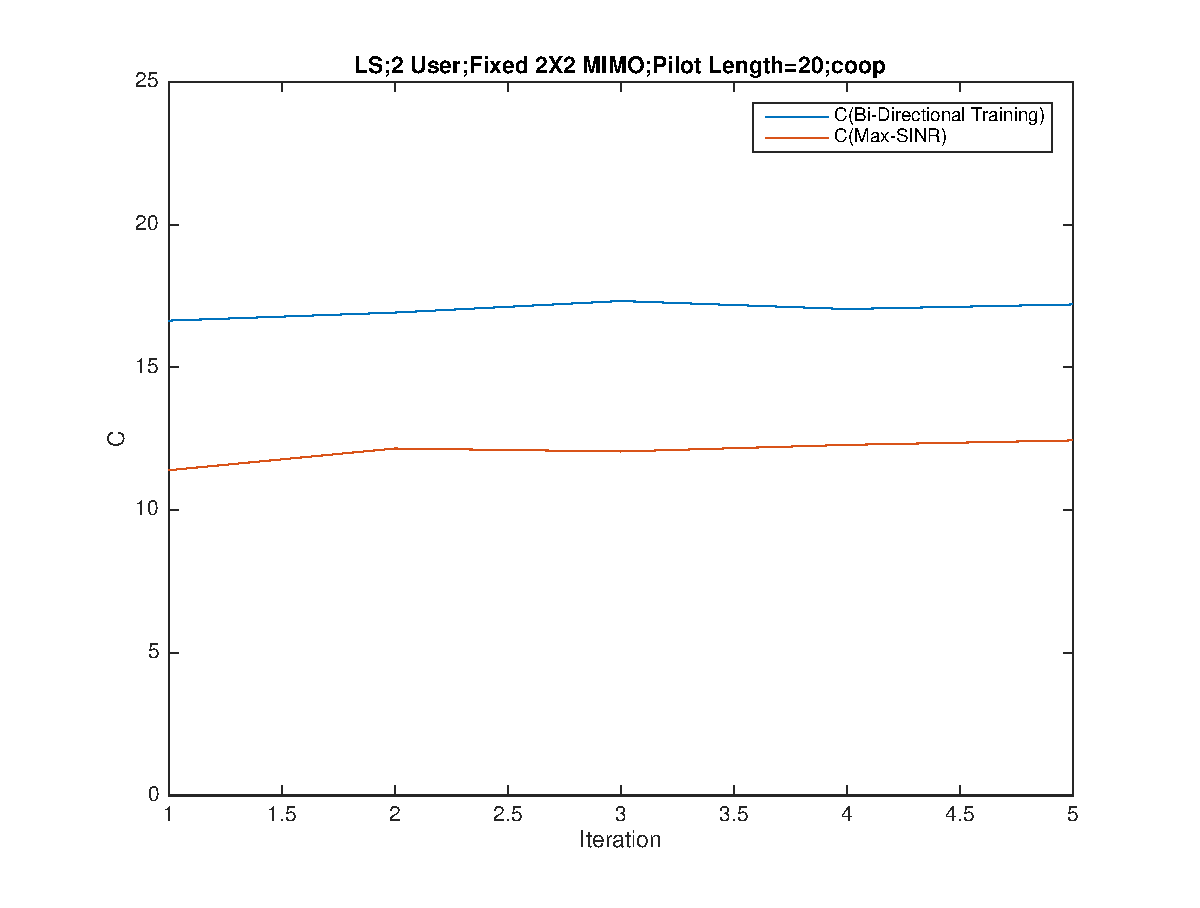
\includegraphics[width=220mm]{coop}}
    \caption{Insert caption}
\end{figure} 

\begin{figure}[bp!]
    \centering
    \centerline{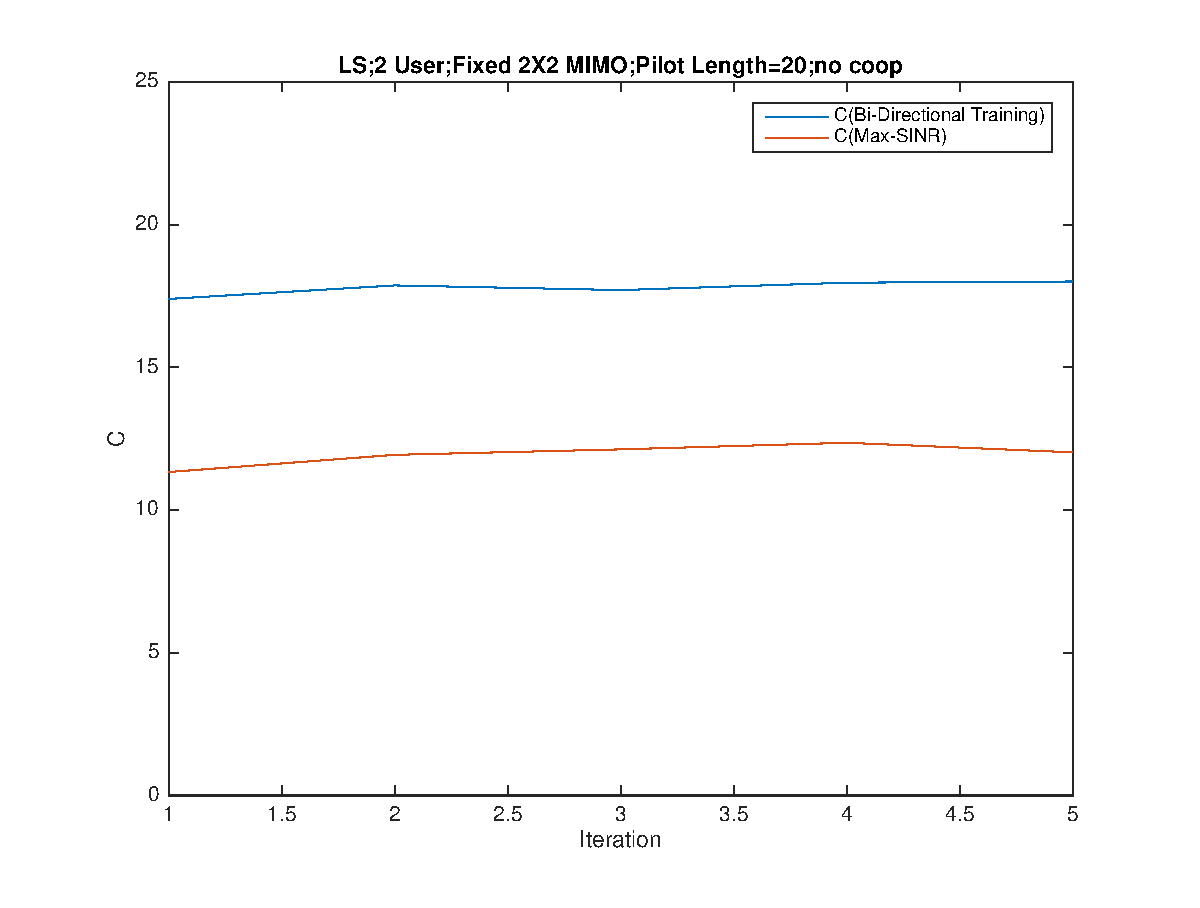
\includegraphics[width=220mm]{no_coop}}
    \caption{Insert caption}
\end{figure} 

 


\end{document}  